\section{Galimi kodo skirstymo į paketus šablonai}
Diskusijose, kaip reikėtų skirstyti programini kodą, paprastai akcentuojami du šablonai - pagal \textit{techninį sluoksnį}, todo: šaltiniai, nurodantys skirstymo būdus
kur kiekvienam funkcionalumui arba kompiuterinės sistemos sluoksniui yra sukuriamas paketas,
grupuojant skirtingų dalykinių sričių esybes, arba pagal \textit{dalykinės srities esybes}, kur vienos esybės kodas, dalykinės srities
esybės funkcionalumas skirtingose programiniuose sluoksniuose yra patalpintas viename pakete.
Tačiau šie du šablonai yra gan platūs ir galėtų būti išskaidyti į daugiau smulkesnių ir tiksliau aprašytų šablonų.
Taip pat, minėtuose šablonuose, būdai kaip ir kodėl skaidyti programinį kodą parinkti akecentuojant tai, kaip programinį
kodą supranta prie jo dirbantys žmonės.
Nuspręsti, kaip žmonės supranta programinį kodą yra gan sudėtingas ir subjektyvus procesas, todėl aprašant šablonus kodo skirstymui
geriau akcentuoti, kaip sugrupuoti paketai bendrauja tarpusavyje ir skirstyti juos pagal klasių naudojimo atvejus ir priklausomybes.
Taip kodo grupavimo metodai yra labiau artimi Martino aprašytiems principams.
Šablonus kaip grupuoti kodą, akcentuojant klasių naudojimo atvejus ir priklausomybes nagrinėja Martin Sandin savo
straipsnyje \textit{Four Strategies for Organizing Code}.
Šis straipsnis idomus tuo, kad autorius nesiplečia į du dažniausiai sutinkamus šablonus - grupuoti pagal techninį sluoksnį arba dalykinės srities esybes,
o aprašo keturis grupavimo būdus arba šablonus, kurie, nors ir įkvėpti minėtų dviejų budų, yra gan unikalūs ir labiau techniškai apibrėžti.


\subsection{Pagal komponentą}
Organizavimas pagal komponentus sumažina sistemos sudėtingumą, pabrėždamas išorinę ir vidinę kodo vienetų darną.
Išorinė darna reiškia, kad paketas turi minimalią sąsają \angl{interface}, kuri atskleidžia tik konceptus (metodus arba duomenų tipus),
kurie yra glaudžiai susiję su komponento teikiama paslauga.
Vidinė darna reiškia, kad pakuotėje esantis kodas yra stipriai susijęs tarpusavyje ir susijęs su teikiama paslauga.

Kodas yra grupuojamas į mažus paketus, turinčius vieną, aiškiai apibrėžtą funkcionalumą ar tikslą, aprašant abstrakciją, kokie paketo elementai
yra pasiekiami iš išorės ir kaip jie naudojami.
Taip sukuriamas kodas, kuris yra lengviau suprantamas.
Tokią kodo grupavimo tvarką sunku palaikyti, tačiau jos rezultatas - kodas, kuris yra lengviau suprantamas, lengviau pagerinamas, lengviau testuojamas
ir, dėl aiškiai aprašytų sąsajų, lengviau pernaudojamas.

\begin{figure}[H]
    \centering
    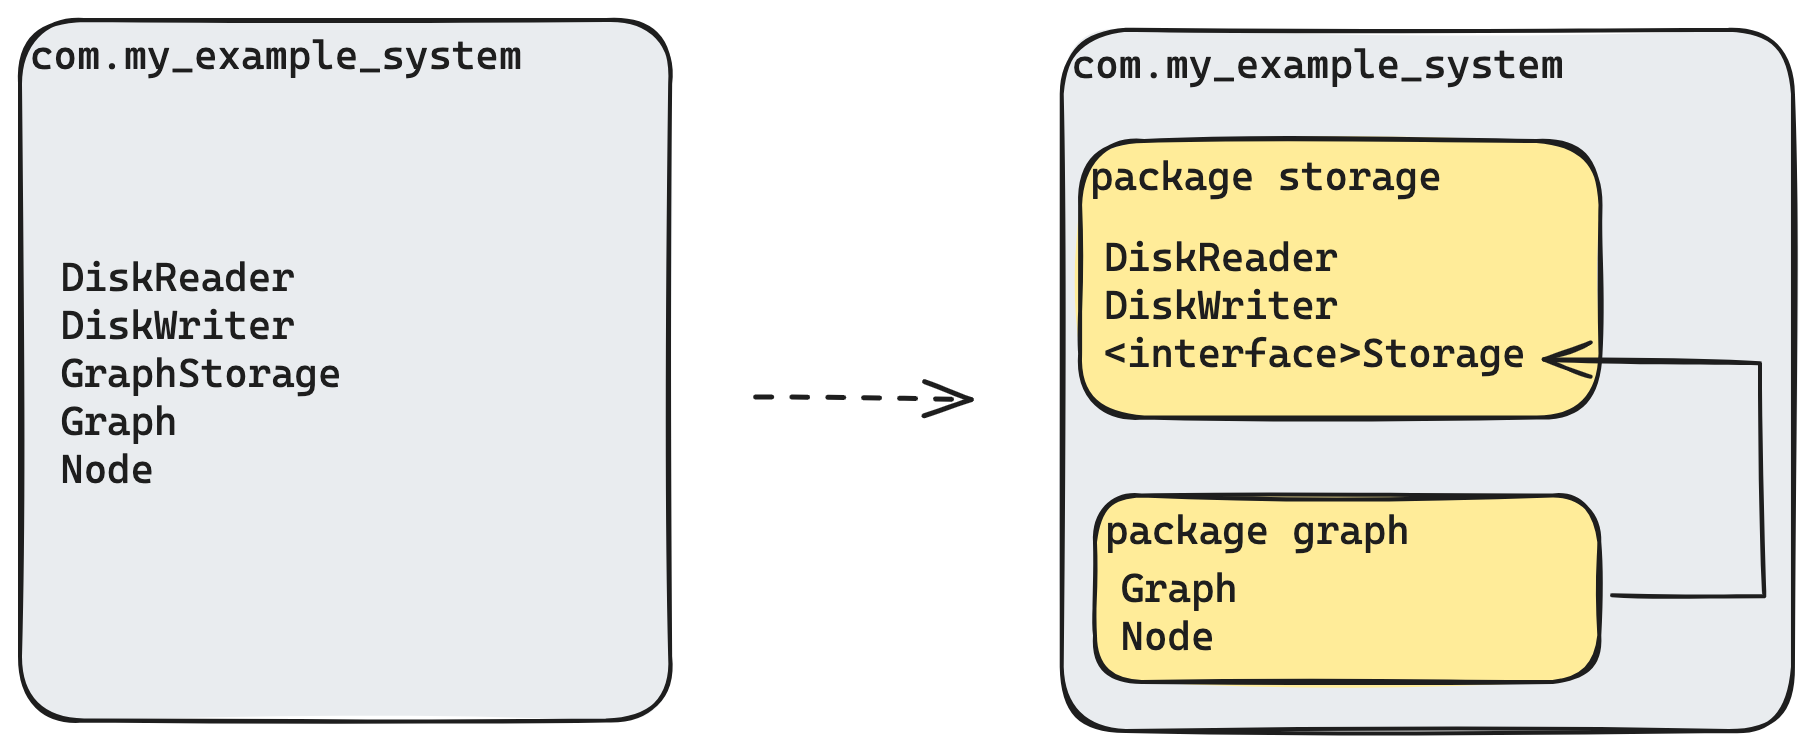
\includegraphics[scale=0.2]{img/component_packaging}
    \caption{Sistemos sugrupuotos pagal komponentą pavyzdys}
    \label{img:component_packaging}
\end{figure}


\subsection{Pagal techninį sluoksnį}
Laikantis skirstymo pagal techninį sluoksnį, kiekvienam funkcionalumui arba kompiuterinės sistemos sluoksniui yra sukuriamas paketas,
kuris savyje grupuoja skirtingas dalykinės srities esybes. Pavyzdžiui, visos sąsajos darbui su duomenų baze guli viename pakete, sąsajos
su verslo logikos transformacijomis kitame, o duomenų vaizdavimo klientui logika trečiame pakete.
Šis paketų skirstymo metodas yra labai paplitęs, ypač tarp senesnių kompiuterinių sistemų. Jį paprasta įgyvendinti,
metode paprasta pavadinti paketus, aišku, į kuriuos paketus priskirti klases. Nors tokią kodo struktūrą lengva įgyvendinti ir palaikyti sistemoje,
ji turi nemažai trūkumų. Šis metodas nepalengvina sistemos plėtros valdymo - augant sistemai paprastai daugėja dalykinės srities esybių,
o ne funkcinių sluoksnių, todėl esamų paketų skaičius beveik nesikeičia, bet klasių kiekis pakete vis auga, tai daro neigiamą įtaką navigacijai
paketo viduje. Skirstant paketus pagal funkciją taip pat nėra gerinamas informacijos slėpimas (inkapsuliacija) - kiekvienas paketas savyje
talpina skirtingų dalykinės srities esybių kodą, tai sudaro salygas per klaidą užmegzti komunikaciją tarp komponentų, kurie neturėtų būti susiję.
Taip pat, skirstant tokiu būdu, sąsajos yra stipresnės tarp loginių komponentų, pasiskirsčiusių per sluoksnius, nei tarp vieno sluoksnio esybių.
Tokiu atveju pokyčių pristatymas pasidaro sudėtingas, nes reikalinga keisti ne vieną sluoksnį.
Tačiau šis metodas turi ne tik trūkumus - vienas iš jo privalumų - ganėtinai aiškiai nusakoma bendra sistemos architektūra, programiniai sluoksniai.
Deja, netvarkinga sistemos būsena eliminuoja ši privalumą.

\subsection{Pagal tipą}
Kodo organizavimas pagal tipą įprastai nėra griežtai apibrėžtas - klasės grupuojamos pagal vartotojo sumanytą tipą, neteikiant svarbos
klasių sąryšiams ar loginėms esybėms. Taip skirstant klases, į paketus galėtų būti grupuojamos esybių, išimčių ar serviso klasės. Šis skirstymo būdas
neteikia prioriteto nei skirstymui pagal techninius sluoksnius, nei pagal dalykinės srities esybes. Jį ganėtinai nesudėtinga įgyvendinti,
tačiau šis metodas yra netvarkingas bei turi trūkumų. Taip suskirstytas kodas sunkiai skaitomas, nes nėra aišku, pagal kokią tvarką
ieškoti konkrečios klasės ar kaip priskirti esamiems paketams netinkamas klases. Taip pat toks skirstymo būdas visiškai nepadeda spręsti
klasių sąsajų problemų, kadangi neapgalvotai išskirstyti sluoksniai gali būti glaudžiai susiję.

\subsection{Pagal funkciją}
Šis skirstymo būdas dalinai panašus į skirstymą pagal komponentą, tačiau yra mažiau griežtas ir
prioritetas teikiamas ne vidinei darnai ir glaudžiai grupuojamų
komponentų sąsajai, o išorinei darnai. Tokio skirstymo būdo paketuose dažniausiai grupuojamos tos pačios sąsajos implementacijos,
parenkamos siekiant pabrėžti išorinę darną ir sugrupuoti klases, teikiančias panašias funkcijas. Toks skirstymas patogus, pavyzdžiui,
techninių bibliotekų vartotojams, kadangi galima lengvai surasti bibliotekos teikiamas funkcijas. Tokią kodo grupavimo tvarką sunku palaikyti,
nes reikia gerai apgalvoti skirstymo strategiją, kad ji būtų prasminga ir patogi naudoti.



\subsection{Problemos}
Aprašant galimus šablonus paketams skirstyti, reikėtų identifikuoti klausimus arba problemas, kurias išspresti gali
gerai sugrupuotas kodas, arba pristatyti / sustiprinti kodas, sugrupuotas neteisingai.

\subsubsection{Kur laikyti pagalbines klases, daugkartinio naudojimo klases?}
Didžiausia problema, susijusi su pagalbinėmis klasėmis, kurios turėtų išspręsti dažnai sistemoje sutinkamas problemas -
inžinieriai, dirbantys prie sistemos nežino apie jų egzistavimą, todėl jų nenaudoja,
tai veda prie didesnio kodo pasikartojimo arba kelių skirtingų to paties pagalbinio funkcionalumo įgyvendinimo.

\begin{figure}[H]
\snugshade
\dirtree{%
    .1 {/} .
    .2 {users} .
    .3 {UserRolesGrouping} .
    .3 {ArrayGroupingHelper} .
    .2 {\ldots} .
    .2 {payments} .
    .3 {PaymentScheduler} .
    .2 {\ldots} .
    .2 {transactions} .
    .3 {TransactionBatching} .
    .3 {utils} .
    .4 {ArrayGroupByUtil} .
}
\endsnugshade
\caption{Sistemos pavyzdys, kur labai panašią funkciją atliekančios klasės \textit{ArrayGroupByUtil} ir \textit{ArrayGroupingHelper}
egzistuoja todėl, kad inžinierius nerado jau įgyvendintos klasės, dėl aiškios struktūros daugartinio
panaudojimo klasėms trūkumo.}
\end{figure}
Vienas iš šablonų, sprendžiančių šią problemą, galėtų būti turėti vieną paketą, skirtą visoms pagalbinėmis klasėmis, kuris yra paminėtas sistemos
dokumentacijoje ir apie jo egzistavimą teoriškai žino visi komandos nariai.
Pakete reikėtų turėti atskiras klases kiekvienam bendriniam domenui, iš kurios pavadinimo programuotojas galėtų nuspresti,
kad jo ieškomas funkcionalumas, bus būtent toje klasėje.

\begin{figure}[H]
\snugshade
\dirtree{%
    .1 {/} .
    .2 {users} .
    .3 {UserRolesGrouping} .
    .2 {\ldots} .
    .2 {payments} .
    .3 {PaymentScheduler} .
    .2 {\ldots} .
    .2 {transactions} .
    .3 {TransactionBatching} .
    .2 {common} .
    .3 {Arrays} .
    .3 {Maps} .
    .3 {SqlQueries} .
    .3 {Users} .
}
\endsnugshade
\caption{Sistemos pavyzdys, kur visas bendrinio panaudojimo kodas guli \textit{common} pakete, pirmame sistemos paketų lygyje, todėl
pagalbinės klasės yra lengvai randamos.}
\end{figure}

Jei pagalbinių klasių dydis labai išauga, jas galima sumažinti ir vietoj vienos atskiros klasės vienai bendrinei sričiai, sukurti vieną paketą,
ir jame turėti kelias pagalbines klases, susijusias su tuo domenu.
Tokiu atveju reikia užtikrinti, kad iš klasių pavadinimo aišku, kokį srities subdomeną padengia klasė.

\begin{figure}[H]
\snugshade
\dirtree{%
    .1 {/common} .
    .2 {arrays} .
    .3 {ArrayFilters} .
    .3 {ArrayComparators} .
    .2 {\ldots} .
    .2 {maps} .
    .3 {MapTransformations} .
    .3 {MapJoining} .
    .2 {json} .
    .3 {JsonParser} .
    .2 {\ldots} .
    .2 {database} .
    .3 {DatabaseConnection} .
    .3 {DatabaseQueries} .
}
\endsnugshade
\caption{Sistemos pavyzdys, kur bendrinio panaudojimo kodas guli \textit{common} pakete, po domeno subpaketais, taip sumažinant klasių dydį }
\end{figure}

Naudojant tokį šabloną, programuotojas, susiduriantis su bendrine problema, kuri, labai tikėtina, jau yra išspresta sistemoje turėtų
aiškų procesą, kaip elgtis šioje situacijoje:
\begin{enumerate}
    \item Atsidaryti vieną paketą, skirtą bendrinio panaudojimo kodui
    \item Pakete surasti klasę, kurios pavadinimas būtų susijęs su jo problema
    \item Klasės funkcijų saraše surasti jam tinkamą funkciją.
    \item Jei reikalingas funkcionalumas nerastas, įgyvendinti jį pasirinktoje klasėje, padengti jį testais,
    bei aprašyti dokumentaciją, kaip funkcija turėtų būti naudojama.
    \item Iškviesti rastą arba sukurtą funkciją iš bendrinio panaudojimo kodo paketo savo funkcionalume
\end{enumerate}

\subsubsection{Ka daryti esant dideliam priklausomybių nuo paketo skaičiui?}
Didelis priklausomybių nuo specifinio paketo skaičius (arba aferentinės jungtys), reiškia, kad pokyčiai tame pakete turės įtaką kelioms klasėms.
Jei tokia tendencija yra būdinga visai sistemai, sistema tampa mažiau lanksti pokyčiams, kadangi net ir paprastas pakeitimas
daro įtaką reišmingai sistemos daliai, pokyčiai yra labiau linkę keisti bendrą sistemos architektūrą.
Taip pat naujos sistemos versijos išleidimo \angl{release} procesas tampa sudetingesnis, kadangi yra paveikiama daugiau klasių.

Robert C. Martin bendro sąryšio principas, kuris teigia, kad visos tarpusavyje susijusios klasės turėtų būti vienam pakete,
akcentuoja siekiamybę turėti gan mažus paketus, turinčius aiškiai apibrėžtą funkcionalumą, priežastį egzistuoti, taip užtikrinant
glaudų tarpusavyje susijusių klasių saryšį.
Šis principas galėtų būti kodo skirstymo šablonas, užtikrinantis racionalų aferentinių jungčių skaičių paketuose.
Vadovaujantis šiuo šablonu kiekvieną paketą reikėtų realizuoti kaip komponentą, teikiantį vieną funkcionalumą,
turintį minimalią sąsają \angl{interface}, kuri atskleidžia tik konceptus (metodus arba duomenų tipus),
kurie yra glaudžiai susiję su komponento teikiama paslauga.

Paketas turintis vieną funkciją yra naudojamas tik tų paketų, kuriems reikia būtent tos funkcijos,
taip užtikrinant tik mažos sistemos dalies priklausomybę nuo vieno paketo.

Taip pat mažas paketo funkcionalumas reiškia, kad minėtas paketas skirtas funkcionalumui įgyvendinti naudos minimalų kitų sistemos esybių skaičių,
taip sumažinant ir eferentinių jungčių skaičių.

Žemiau esančiuose paveikslėliuose galima matyti, kaip išskaidant paketus, turinčius kelis funckionalumus, yra sumažinamas paketų
priklausomybių skaičius.
\begin{figure}[H]
    \centering
    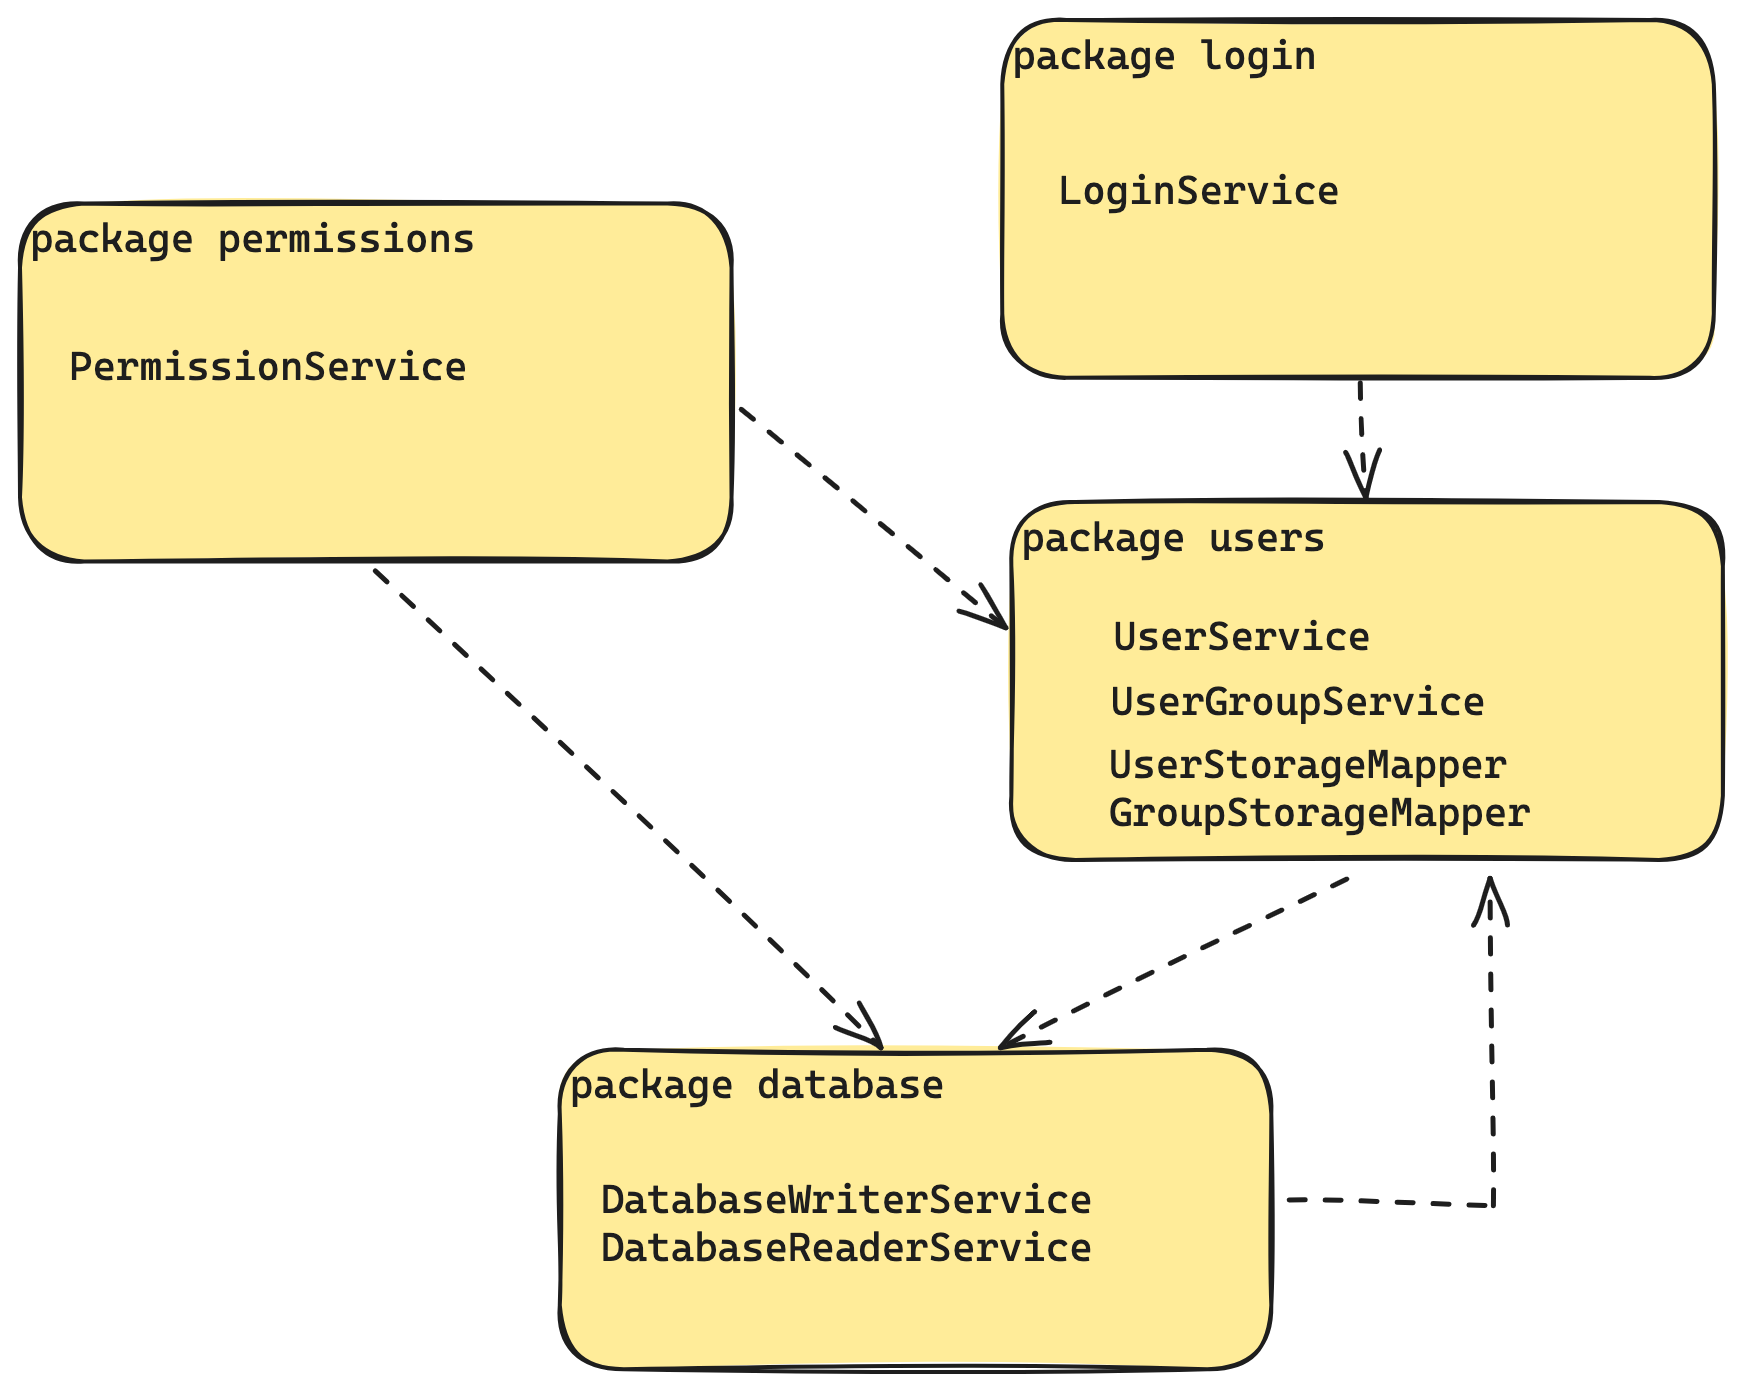
\includegraphics[scale=0.15]{img/excesive_deps}
    \caption{Sistemos pavyzdys su kelias funkcijas atliekančiais paketais}
    \label{img:excesive_deps}
\end{figure}


\begin{figure}[H]
    \centering
    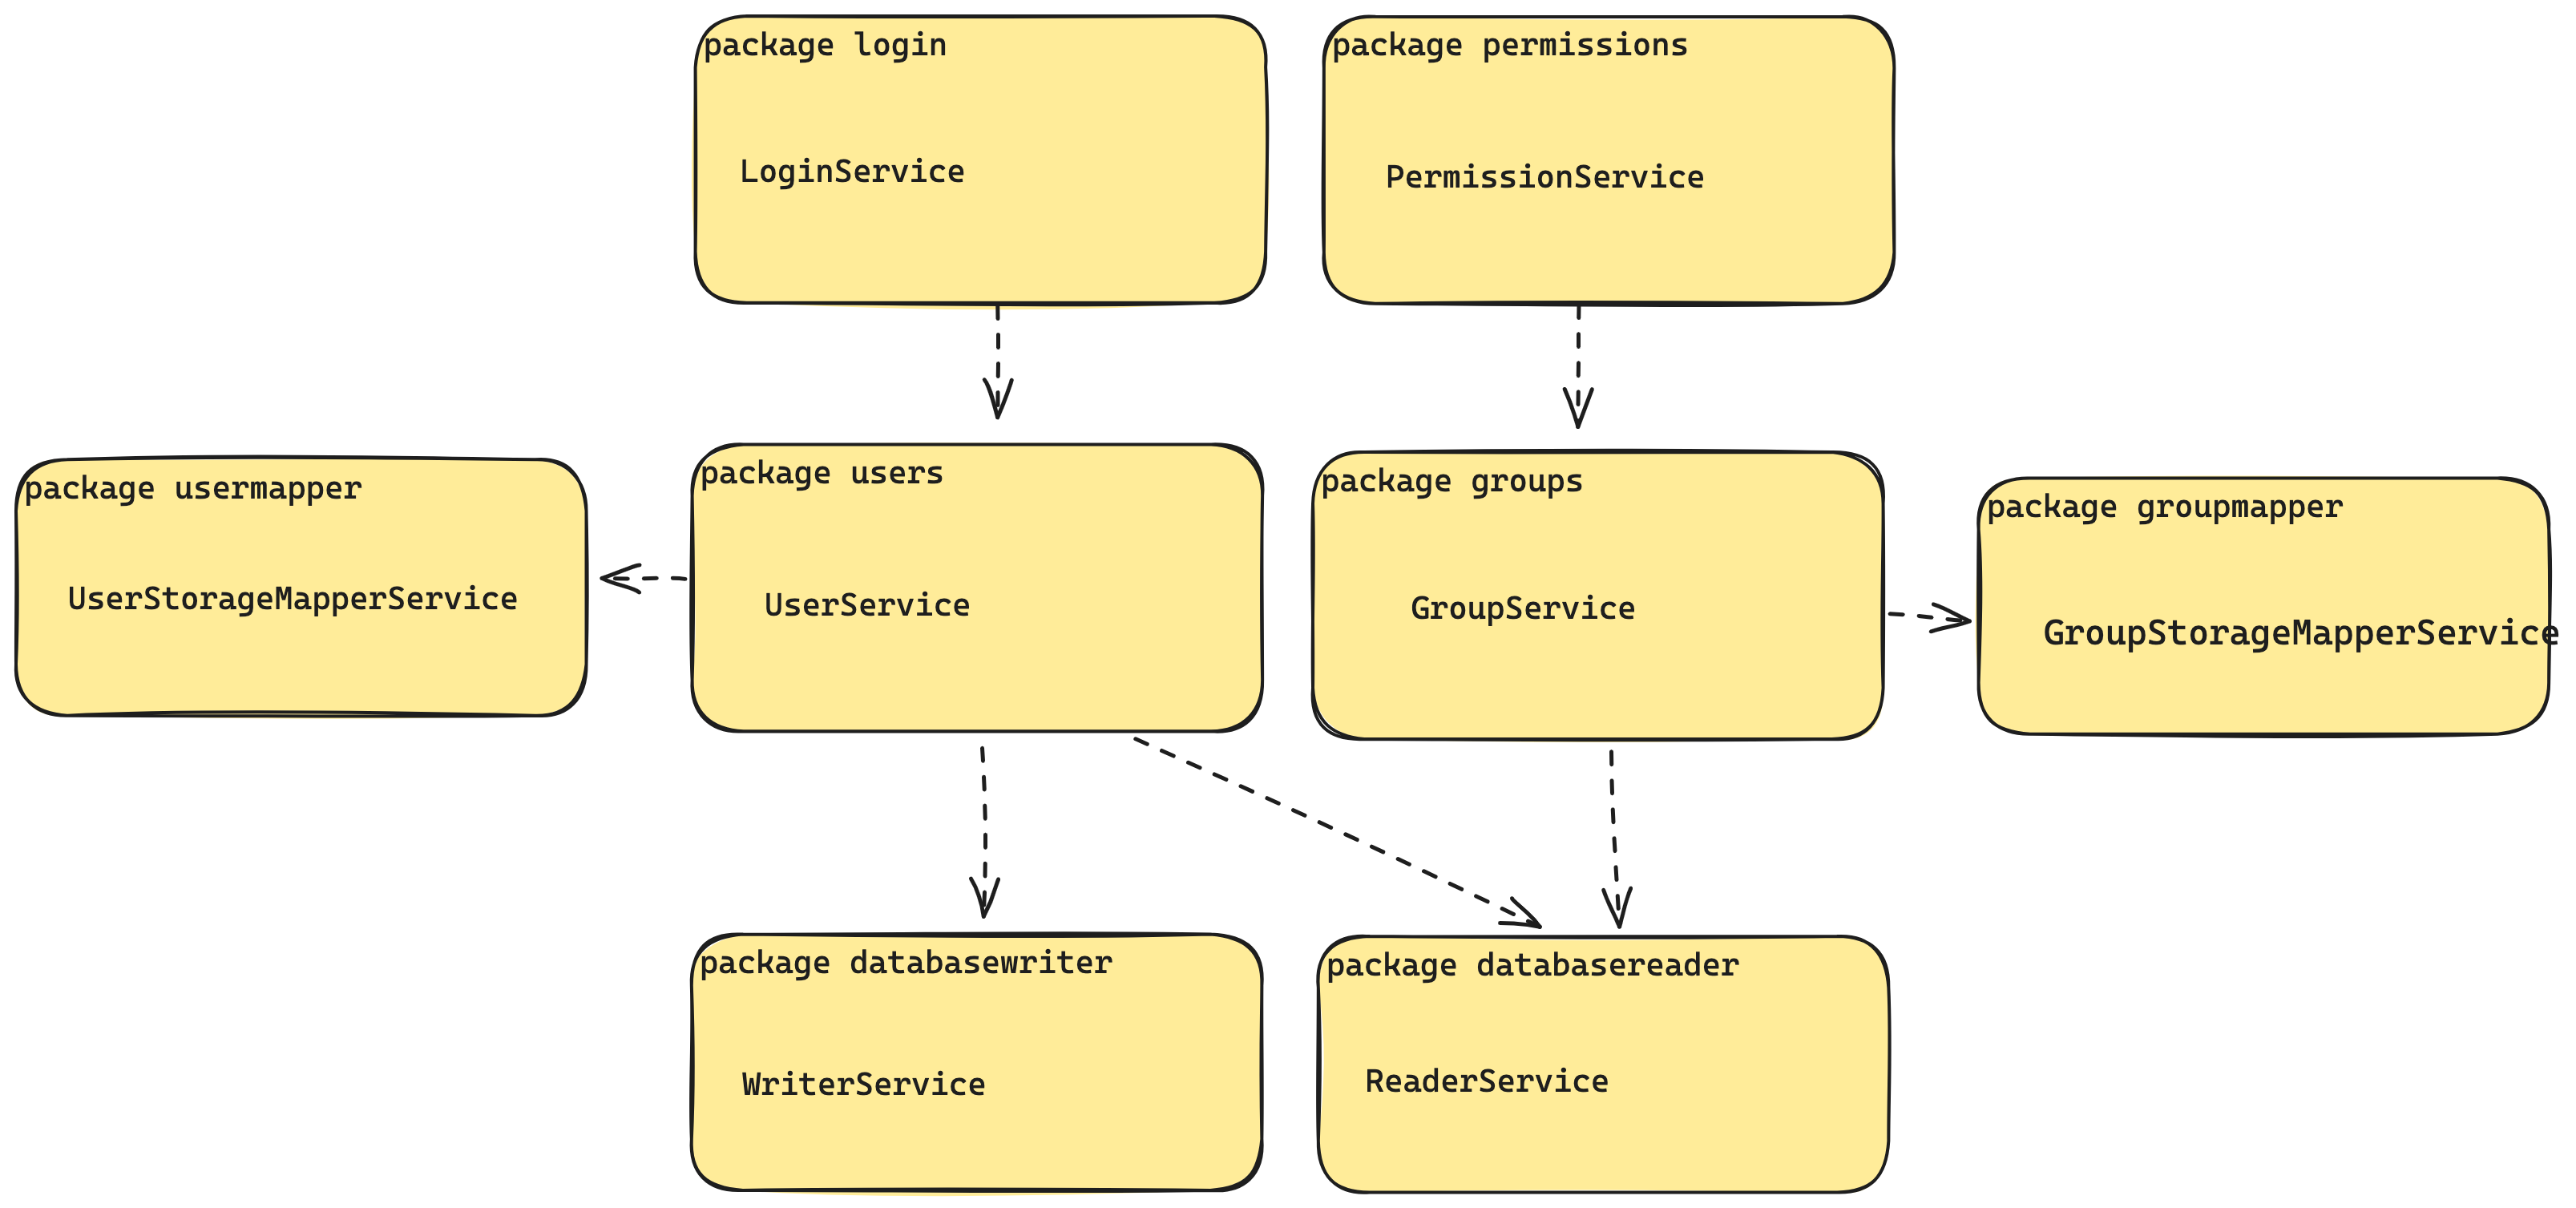
\includegraphics[scale=0.13]{img/good_deps}
    \caption{Sistemos pavyzdys su aiškią, vieną funkciją turinčiais paketais}
    \label{img:good_deps}
\end{figure}


\subsubsection{Ka daryti su ciklinėmis priklausomybėmis?}

\subsubsection{Ka daryti su daug skirtingų sąsajų implementacijų?}
\subsubsection{Ka daryti su mikroservisų architektūra?}
\subsubsection{Ka daryti su pasleptom priklausomybem?}
\subsubsection{Kaip grpuoti kodą mono repozitorijoj?}
\subsubsection{Ka daryti greitai besikeičiančių kodu?}
\subsubsection{Ka valdyti esybių evoliuciją ir versijavimą}






Packaging microservice classes involves structuring your codebase in a way that promotes modularity, scalability, and maintainability within the microservices architecture. Here's how you can package microservice classes effectively:


2. *Separate Concerns*:
- Follow the single responsibility principle (SRP) by separating concerns within each package.
- For example, separate classes responsible for handling HTTP requests, business logic, data access, and external integrations into distinct packages or modules.


5. *API Contract Packaging*:
- Define clear API contracts for your microservices, specifying the expected inputs, outputs, and behavior of each service.
- Group classes related to API endpoints, request/response models, and error handling into dedicated packages representing the API contract.

6. *Infrastructure Concerns*:
- Separate infrastructure-related concerns, such as database access, caching, logging, and messaging, into their own packages or modules.
- This helps isolate infrastructure-specific code and configurations, making it easier to maintain and evolve over time.

code duplication


8. *Testing Concerns*:
- Organize test classes alongside production code, following a similar package structure.
- Group unit tests, integration tests, and end-to-end tests into separate packages or modules to maintain clarity and organization.

3. *Difficulty in Understanding and Navigation*:
- Unorganized code makes it hard for developers to understand the structure and relationships between different parts of the system.
- Lack of clear packaging boundaries makes navigation and code exploration challenging, especially for new team members or maintainers.


To solve the problem of multiple interface implementations, you can use several packaging techniques. Here are some approaches:

1. *Interface Segregation Principle (ISP)*:
- Follow the ISP, one of the SOLID principles, by segregating interfaces based on client requirements.
- Instead of having a single interface with multiple methods, create smaller, more focused interfaces with a single responsibility.
- Group related methods into separate interfaces, allowing classes to implement only the interfaces that are relevant to them.

2. *Package by Feature*:
- Organize classes implementing related interfaces into packages based on feature or functionality.
- Each package contains classes that provide a specific feature and implement the necessary interfaces for that feature.
- This approach keeps related classes together and reduces the likelihood of conflicts between different interface implementations.

5. *Factory Pattern*:
- Use the factory pattern to create instances of classes implementing specific interfaces.
- Define factory methods or classes that encapsulate the logic for instantiating different implementations of an interface.
- This centralizes the creation logic and allows for dynamic selection of implementations based on runtime conditions.

6. *Composition over Inheritance*:
- Prefer composition over inheritance when designing class relationships.
- Instead of implementing multiple interfaces directly in a single class, consider composing the class of multiple smaller components, each implementing a specific interface.
- This promotes flexibility, as you can mix and match components to achieve different behaviors without creating complex inheritance hierarchies.

1. *Modularity*: Packaging allows breaking down a large system into smaller, more manageable modules. This enhances modularity, making it easier to understand, maintain, and extend the codebase.



4. *Code Reusability*: Well-packaged code promotes code reuse by encapsulating reusable components or libraries into separate packages. This reduces duplication and improves overall productivity.

6. *Collaboration*: Packaging encourages collaboration among team members by providing clear boundaries between different parts of the system. It enables parallel development and reduces the risk of conflicts when multiple developers work on the same project.





Could you give patterns how to group code into packages:

Certainly! Grouping code into packages is a common practice in many programming languages to organize and manage large codebases effectively. Here are some patterns for grouping code into packages:

1. *Functional Grouping*:
- Group code based on functionality or domain. For example, in a web application, you might have packages like authentication, user-management, payment, etc.
- Each package contains related modules, classes, or functions that handle specific tasks within that domain.

2. *Layered Architecture*:
- Organize code into layers such as presentation, business logic, and data access layers.
- Each layer represents a different aspect of the application, with well-defined responsibilities and dependencies.

3. *Feature-Based Packaging*:
- Group code based on features or components of the application.
- Each feature or component has its own package containing all the necessary code, including UI, logic, and data handling.

4. *Namespace Packaging*:
- Use namespaces or packages to organize code based on hierarchical relationships.
- For example, in Java, you might have packages like com.example.project.module1, com.example.project.module2, etc.

5. *Modular Packaging*:
- Divide the application into smaller, independent modules that can be developed, tested, and deployed separately.
- Each module may contain its own set of packages, making it easier to manage dependencies and promote code reuse.

6. *Aspect-Oriented Packaging*:
- Separate cross-cutting concerns such as logging, security, and caching into their own packages.
- These packages can then be applied to different parts of the application as needed, using techniques like aspect-oriented programming (AOP).

7. *Dependency Injection Packaging*:
- Organize code based on the dependency injection (DI) hierarchy.
- Group classes and components that depend on each other closely within the same package to facilitate DI configuration and management.

8. *Component-Based Packaging*:
- Treat each component of the application as a standalone unit with its own package.
- Components may include UI widgets, services, data models, etc., each residing in its own package for easier maintenance and reuse.

By applying these packaging patterns, you can create a well-organized codebase that is easier to understand, maintain, and extend over time